\section[تمرین سوم - سوال دوم: ترکیب VAE و Normalizing Flows]{\faProjectDiagram\ \ تمرین سوم - سوال دوم: ترکیب \lr{Variational Autoencoders} و \lr{Normalizing Flows}}

\begin{stepbox}

\field{هدف مساله}{
در این سوال قصد داریم با استفاده از مفهوم جریان‌های نرمال‌ساز (\lr{Normalizing Flows})، انعطاف‌پذیری و قدرت مدل‌سازی فضای پنهان (\lr{Latent Space}) را در مدل‌های \lr{VAE} افزایش دهیم. در \lr{VAE} استاندارد، توزیع پیشین (\lr{Prior}) معمولاً یک توزیع گاوسی ساده فرض می‌شود که برای بازنمایی داده‌های پیچیده محدودیت ایجاد می‌کند. با اعمال دنباله‌ای از نگاشت‌های معکوس‌پذیر، این توزیع ساده به توزیع‌های پیچیده‌تر و چندوجهی تبدیل می‌شود. در این تمرین، عملکرد این ایده روی مجموعه داده \lr{FashionMNIST} مورد بررسی و ارزیابی قرار گرفته است.
}

\field{بصری‌سازی داده‌های ورودی (\lr{FashionMNIST})}{
در ابتدای کار، یک بچ (Batch) ثابت از داده‌های تست برای ارزیابی کیفی مدل‌ها انتخاب شد. مجموعه داده \lr{FashionMNIST} شامل تصاویر ۲۸×۲۸ پیکسل سیاه‌وسفید از پوشاک (نظیر کفش، کیف، تیشرت و...) است. شکل زیر نمونه‌ای از این داده‌های ورودی را نشان می‌دهد که قرار است مدل‌های ما یاد بگیرند آن‌ها را بازسازی کنند.

\vspace{0.4cm}

\begin{center}
    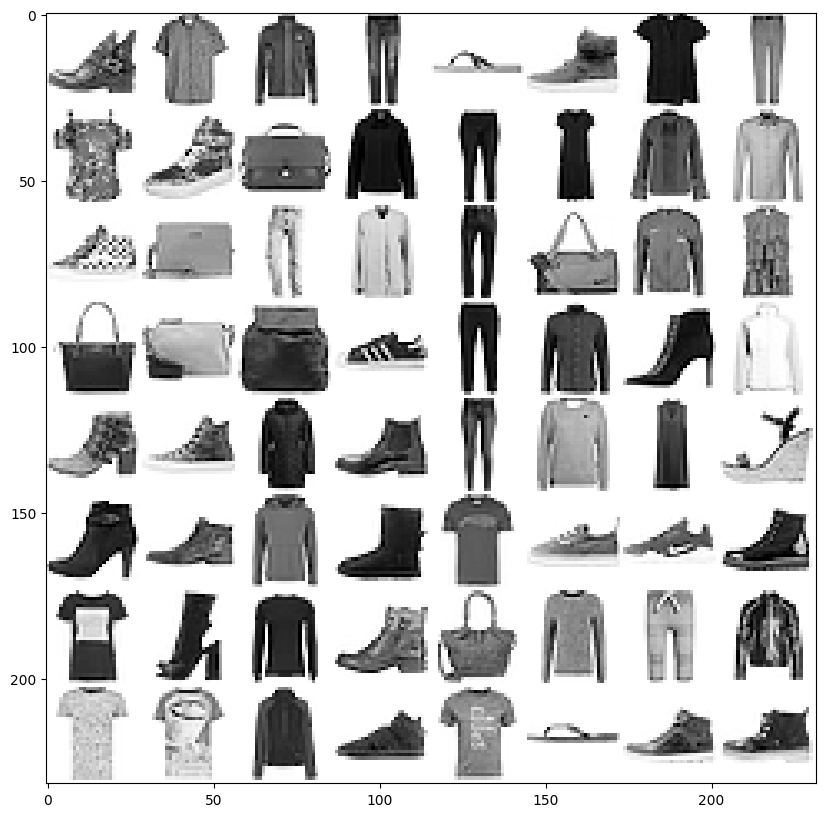
\includegraphics[width=0.55\textwidth]{images/original_batch.png} % عکس داده‌های اولیه
    \captionof{figure}{نمونه‌ای از داده‌های ورودی مجموعه \lr{FashionMNIST}}
\end{center}
}

\field{تحلیل روند آموزش و خطای بازسازی (\lr{Loss})}{
در فرآیند آموزش مدل‌ها، تابع هزینه شامل دو بخش اصلی است: خطای بازسازی (images/Reconstruction Loss) برای سنجش کیفیت تصاویر تولید شده، و یک عبارت تنظیم‌کننده (مانند KL Divergence یا Variational Free Energy) برای ساختاردهی به فضای پنهان.
همان‌طور که در نمودار زیر مشاهده می‌شود، خطای آموزش در اپوک‌های اولیه با شیب تندی کاهش یافته و سپس به یک پایداری نسبی می‌رسد. نوسانات جزئی در نمودار به دلیل استفاده از زیرمجموعه‌های تصادفی (Subsampling) در هر اپوک است. 

\vspace{0.4cm}

\begin{center}
    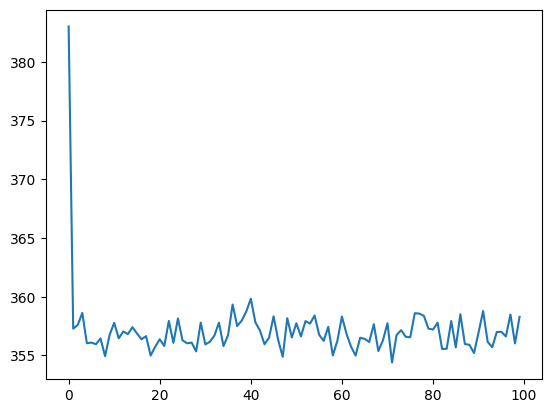
\includegraphics[width=0.65\textwidth]{images/loss_plot.png} % عکس نمودار Loss
    \captionof{figure}{روند کاهش خطای بازسازی در طول تکرارهای آموزش}
\end{center}
}

\field{کیفیت بازسازی تصاویر (Reconstructions)}{
در طول فرآیند آموزش، مدل‌ها سعی کردند تصاویر بچ ثابت (Fixed Batch) را بازسازی کنند. در تکرارهای اولیه، خروجی مدل‌ها صرفاً هاله‌ای تار و نویزدار از تصاویر بود. اما با پیشرفت آموزش، مدل‌ها توانستند ساختار کلی اشیاء (مانند فرم کلی کفش یا کیف) را یاد بگیرند. 
در مقایسه بین مدل‌ها، مدل‌هایی که به جریان نرمال‌ساز مجهز بودند (\lr{Planar Flow})، توانستند جزئیات و لبه‌های تصاویر را با وضوح بهتری نسبت به \lr{Vanilla VAE} بازسازی کنند.

\vspace{0.4cm}

\begin{center}
    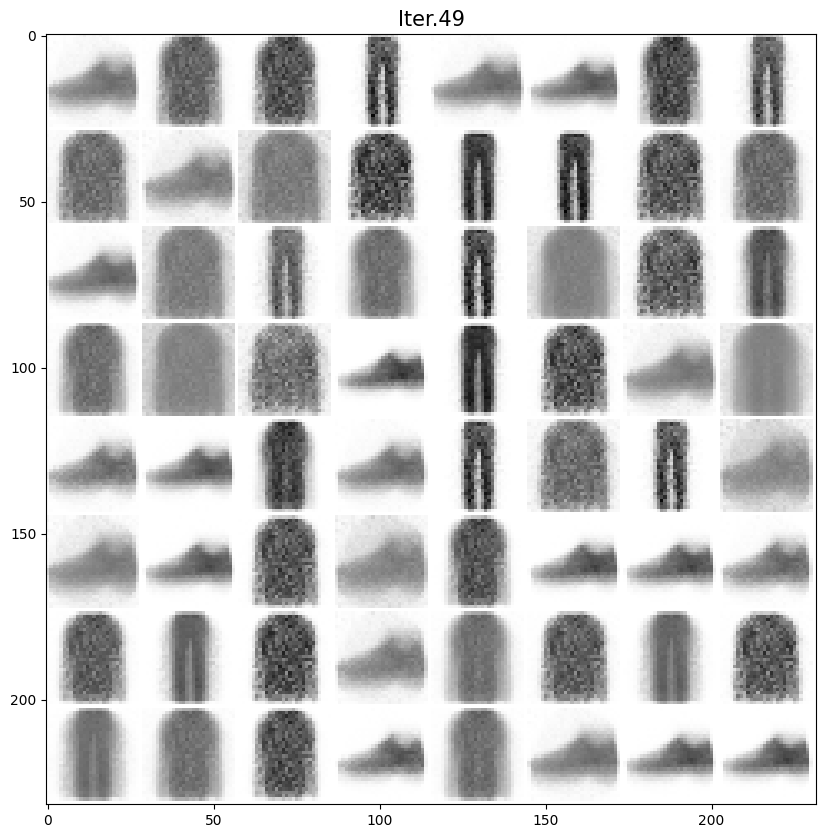
\includegraphics[width=0.55\textwidth]{images/reconstructed.png} % عکس بازسازی نهایی
    \captionof{figure}{خروجی بازسازی شده تصاویر توسط مدل پس از اتمام آموزش}
\end{center}
}

\field{تحلیل فضای پنهان (\lr{Latent Space}) و مقایسه سه مدل}{
مهم‌ترین بخش این تمرین، بررسی تاثیر افزودن \lr{Flow} به فضای پنهان است. برای این منظور، سه ساختار مختلف پیاده‌سازی شدند و خروجی آن‌ها توسط الگوریتم کاهش ابعاد \lr{PCA} (به دو بُعد) تصویرسازی شد:

\begin{itemize}
    \item \textbf{حالت اول - \lr{Vanilla VAE}:} در این حالت (نمودار سمت چپ)، به دلیل استفاده از یک توزیع نرمال ساده، کلاس‌های مختلف به شدت درهم‌تنیده هستند و مرز مشخصی بین کلاسترها وجود ندارد. مدل در جداسازی ویژگی‌های پوشاک مختلف ضعیف عمل کرده است.
    
    \item \textbf{حالت دوم - \lr{Planar Independent}:} با اضافه شدن جریان‌های متوالی به توزیع پنهان (نمودار وسط)، توزیع از حالت گاوسی خارج شده و منعطف‌تر شده است. در اینجا کلاسترها (گروه‌های رنگی مشابه) فشردگی بهتری پیدا کرده‌اند و تداخل کلاس‌های نامرتبط تا حد قابل توجهی کاهش یافته است.
    
    \item \textbf{حالت سوم (نمره امتیازی) - \lr{Planar Params / Amortized Inference}:} در این حالت پیشرفته (نمودار سمت راست)، پارامترهای جریان نرمال‌ساز ایستا نیستند و شبکه‌ی انکودر متناسب با هر تصویر، پارامترهای اختصاصی \lr{Flow} مربوط به آن را پیش‌بینی می‌کند. همان‌طور که مشخص است، این حالت بهترین تفکیک‌پذیری را ایجاد کرده است. کلاس‌های هم‌خانواده با تراکم بسیار بالا در کلاسترهای کاملاً مجزا و جزیره‌ای قرار گرفته‌اند. همچنین ارزیابی \lr{NLL} (Negative Log-Likelihood) نیز نشان می‌دهد که این مدل کمترین میزان خطا را در مدل‌سازی توزیع داده‌ها داشته است.
\end{itemize}

\vspace{0.4cm}

\begin{center}
    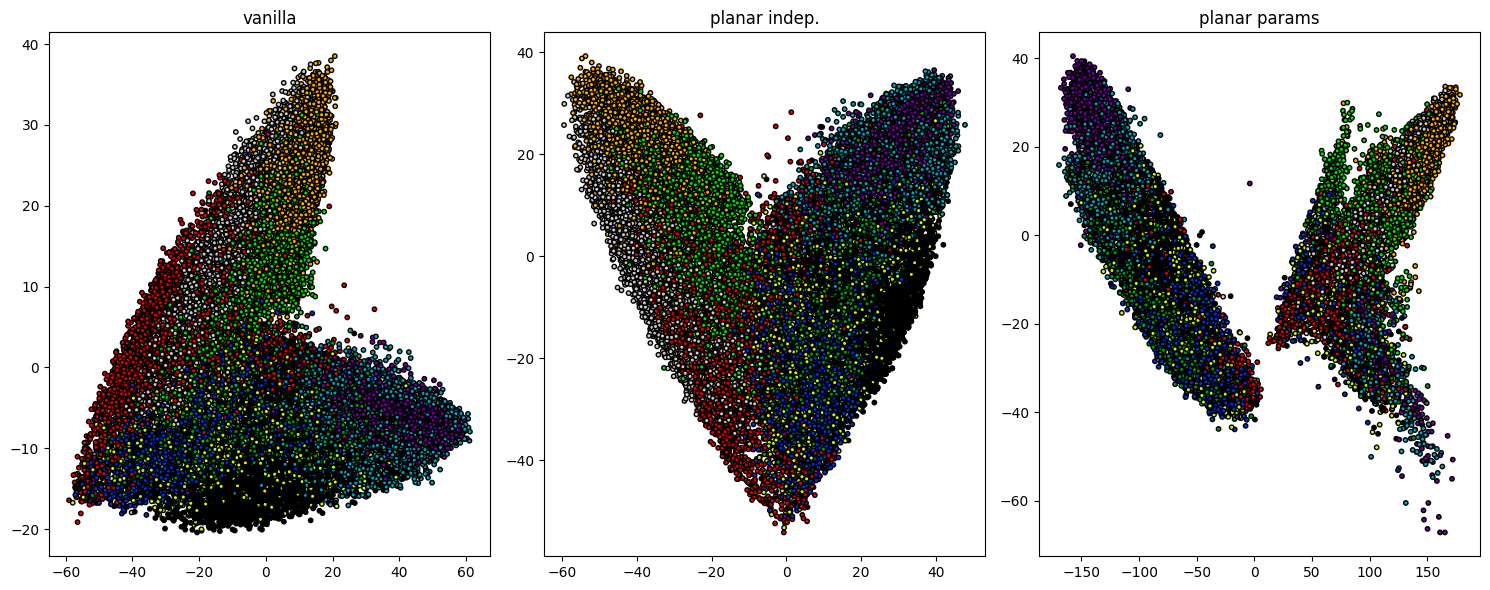
\includegraphics[width=0.95\textwidth]{images/pca_output.png} % عکس نمودارهای PCA
    \captionof{figure}{مقایسه فضای پنهان استخراج شده توسط مدل‌های مختلف با استفاده از الگوریتم PCA}
\end{center}
}

\end{stepbox}